
%% Definição de problema multi-objectivo

Em problemas reais é comum a existência de situações nas quais se
deseja otimizar mais de um objetivo, geralmente conflitantes.
Estes problemas são chamados multiobjetivos e,
diferentemente dos problemas de otimização escalar,
não possuem uma solução melhor, mas várias
soluções de interesse, chamadas \emph{soluções eficientes}.

Um problema de otimização multiobjetivo com $\np$ objetivos pode ser descrito como uma
função vetorial $f(x) = \big(f_1(x), \ldots, f_{\np}(x)\big)$
para a qual se deseja encontrar vetores $x \in X$
que maximizem simultaneamente as $\np$ funções objetivo.
Formalmente:
\begin{align*}
  \text{max} ~ f(x) &=
    \big(f_1(x)
    ,f_2(x)
    ,\ldots
    ,f_{\np}(x)\big) \\
  \text{sujeito a} \quad & x \in X
\end{align*}

A seguir são apresentadas algumas definições importantes, relacionadas a problemas multiobjetivo,
necessárias para o desenvolvimento do presente trabalho.

\begin{mydef}[Dominância, Eficiência e \paretoset{}]
Considere um problema de otimização multiobjetivo.
Diz-se que uma solução $x \in X$
\emph{domina} uma solução $y \in X$, denotado por $x \dom y$
se, e somente se, $x$ é ao menos tão boa quanto
$y$ em todos os objetivos e melhor que $y$ em ao menos um dos objetivos.
Formalmente:
\begin{equation}
    x \dom y \iff \left\{
      \begin{array}{l}
          \forall i \in \{1, 2, \ldots, \np\}: f_i(x) \geq f_i(y) ~\text{e}\\
          \exists j \in \{1, 2, \ldots, \np\}: f_j(x) > f_j(y)
  \end{array} \right.
  \label{eq:dom}
\end{equation}
Uma solução $x \in X$ é dita \emph{eficiente}, denotado por $\text{eff}(x)$,
se, e somente se, $x$ não é dominada por nenhuma outra solução pertencente a $X$.
Formalmente:
\begin{displaymath}
  eff(x) \iff \nexists \big(y \in X \wedge y \dom x \big)
\end{displaymath}

O conjunto de todas as soluções eficientes de um problema multiobjetivo,
denotado por $Par(X)$, é chamado de \emph{\paretoset{}} ou \emph{\paretosetII{}}.
Formalmente:
\begin{displaymath}
  Par(X) = \{ x \in X \;|\; \text{eff}(x)\}
\end{displaymath}
\end{mydef}

Resolver um problema multiobjetivo consiste em determinar seu \paretoset{}.
Este conceito foi primeiramente elaborado por Vilfredo Pareto em 1896, que
enunciou a relação Pareto-Ótima que diz: ``não é possível melhorar uma característica
do problema sem piorar outra'', o que caracteriza a relação conflitante entre os
objetivos na otimização multiobjetivo.

A Figura~\ref{fig:dom-def} ilustra o conceito de dominância de um problema multiobjetivo.
A solução $x$ em destaque domina todas as soluções sob a área hachurada
por estas se identificarem com a Equação~\ref{eq:dom}.
A Figura~\ref{fig:eff-def} ilustra o conceito de conjunto Pareto.
As soluções sobre o traçado em destaque representam um \paretoset{} por
dominarem todas as outras soluções sob a área hachurada.

\begin{figure}[H]
    \centering
    \begin{subfigure}[t]{0.3\textwidth}
        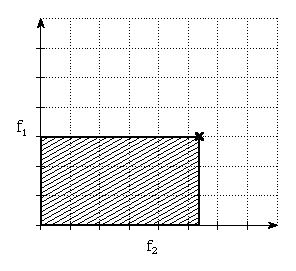
\includegraphics[width=\textwidth]{img/mokp/dom-def}
        \caption{Região de dominância de uma solução.}
        \label{fig:dom-def}
    \end{subfigure}
    \qquad
    \begin{subfigure}[t]{0.3\textwidth}
        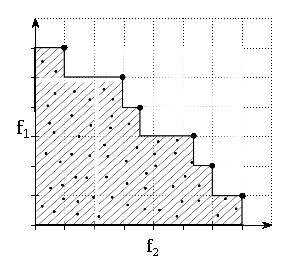
\includegraphics[width=\textwidth]{img/mokp/pareto-def}
        \caption{Exemplo de \paretoset{}.}
        \label{fig:eff-def}
    \end{subfigure}
    \caption{Exemplos de solução dominante e \paretoset{}.}
    \label{fig:mo-defs}
\end{figure}

Convém ressaltar que para problemas multiobjetivo não existe, ou é desconhecida,
qualquer função que agregue os valores de objetivo em um único valor,
caso contrário, o problema poderia ser tratado como um problema de 
otimização escalar.
Sendo assim, a decisão de qual solução será utilizada,
ou quais soluções serão utilizadas, está fora do escopo de resolução.

%%%%%%%%%%%%%%%%%%%%%%%%%
%%% Definição do MOKP %%%
%%%%%%%%%%%%%%%%%%%%%%%%%
Um dos problemas multiobjetivos mais estudados
é o problema da mochila multiobjetivo, \emph{multiobjective knapsack problem} em inglês (\mokp{}).
Diversos problemas reais podem ser modelados como uma instância do \mokp{}, tais 
como seleção de projetos~\cite{teng1996multiobjective},
orçamento de capital~\cite{rosenblatt1989generating},
carregamento de carga~\cite{teng1996multiobjective}
e planejamento de estoque~\cite{ishibuchi2015behavior}.

Uma instância de um problema da mochila multiobjetivo com $\np$
objetivos consiste em uma capacidade inteira $W >0$ e $n$ itens.
Cada item $i$ possui um peso inteiro positivo $w_i$ e $\np$ lucros inteiros
$p_i^1, p_i^2, \ldots, p_{i}^{\np}$ não negativos,
sendo $p_i^k$ a contribuição do $i$-ésimo item para com o $k$-ésimo objetivo.
Uma solução é representada por um vetor binário $\sol{x} = (x_1, \ldots, x_n)$
tal que $x_k = 1$ representa a inclusão do $k$-ésimo item na mochila e $x_k = 0$
representa o caso contrário.
Uma solução é viável se o peso total incluído na mochila não ultrapassa
a capacidade da mochila.
Formalmente a definição do problema é a seguinte:
\begin{align*}
  \text{max   } & f(x) =
    \big(f_1(x) ,f_2(x) ,\ldots ,f_{\np}(x)\big) \\
  \text{sujeito a   } & w(x) \leq W \\
  & x \in \{0, 1\}^n\\
  \text{onde} \phantom{mmmmm} \\
  %I_n &= \{1, \ldots, n\}\\
  f_j(x) &= \sum_{i = 1}^n p^j_i x_i \quad j = 1, \ldots, \np\\
  w(x) &= \sum_{i = 1}^n w_i x_i
\end{align*}

O \mokp{} é considerado um problema \nphard{} visto ser uma generalização
do clássico problema da mochila $0-1$, para o qual $\np = 1$~\cite{garey2002computers}.
É consideravelmente difícil determinar o \paretoset{} para um \mokp{},
pois este tende a crescer rapidamente com o tamanho do problema,
especialmente com o número de objetivos~\cite{ishibuchi2008evolutionary}.
Até mesmo para casos bi-objetivos, problemas relativamente pequenos podem se apresentar
inviáveis.

A Tabela~\ref{tab:exinst} apresenta um exemplo de instância para o MOKP
com $2$ objetivos e $10$ itens, com valores de peso e lucro entre $0$ e $9$ e capacidade
de mochila $W = 28$.
A Tabela~\ref{tab:exsol} apresenta o conjunto Pareto da instância.
Vale observar através da Tabela~\ref{tab:exsol} a potencial complexidade do problema que, neste caso,
possui $6$ soluções eficientes, sendo uma instância de apenas $10$ itens.
Vale observar também o caráter único das soluções eficientes:
se considerarmos a solução $x_{3}$, por exemplo, nenhuma solução
possui simultaneamente $f_1$ maior que $32$ e $f_2$ maior que $34$, caso contrário,
a solução $x_{3}$ poderia ser descartada.

\begin{table}[ht]
  \begin{center}
  \begin{tabular}{|r*{10}{|c}|cc||cc}
  \cline{1-11}
  
    & \multicolumn{10}{c|}{Itens} \\ \cline{1-11}
      & \textbf{1} & \textbf{2} & \textbf{3} & \textbf{4} & \textbf{5} & \textbf{6} & \textbf{7} & \textbf{8} & \textbf{9} & \textbf{10} \\ \cline{1-11}
    \textbf{$\boldsymbol{p^1}$} & 4 & 9 & 3 & 1 & 8 & 7 & 2 & 5 & 6 & 7  \\ \cline{1-11}
    \textbf{$\boldsymbol{p^2}$} & 8 & 4 & 2 & 2 & 3 & 0 & 6 & 8 & 9 & 6  \\ \cline{1-11} \cline{13-14}
    \textbf{$\boldsymbol{w}$}   & 7 & 8 & 5 & 8 & 3 & 5 & 6 & 2 & 4 & 9
        & & \multicolumn{1}{|c|}{$\boldsymbol{W}$}
        & \multicolumn{1}{c|}{28}\\ \cline{1-11} \cline{13-14}
  \end{tabular}
\end{center}
  \caption{Exemplo de instância do problema da mochila bi-objetivo com $10$ itens.}
  \label{tab:exinst}
\end{table}

\begin{table}[ht]
  
\begin{center}
  \begin{tabular}{|c*{10}{|c}||c|c|c|c|}
    \cline{2-14}
    \multicolumn{1}{c|}{}
      & \textbf{1}
      & \textbf{2}
      & \textbf{3}
      & \textbf{4}
      & \textbf{5}
      & \textbf{6}
      & \textbf{7}
      & \textbf{8}
      & \textbf{9}
      & \textbf{10}
      & $\boldsymbol{f_1}$
      & $\boldsymbol{f_2}$
      & $\boldsymbol{w}$ \\ \hline
    \textbf{$\boldsymbol{x_{1}}$} & \bc &     &     &     &     &     & \bc & \bc & \bc & \bc & 24 & 37 & 28 \\ \hline
    \textbf{$\boldsymbol{x_{2}}$} & \bc &     & \bc &     & \bc &     & \bc & \bc & \bc &     & 28 & 36 & 27 \\ \hline
    \textbf{$\boldsymbol{x_{3}}$} & \bc &     &     &     & \bc & \bc & \bc & \bc & \bc &     & 32 & 34 & 27 \\ \hline
    \textbf{$\boldsymbol{x_{4}}$} &     & \bc & \bc &     & \bc &     & \bc & \bc & \bc &     & 33 & 32 & 28 \\ \hline
    \textbf{$\boldsymbol{x_{5}}$} &     & \bc &     &     & \bc & \bc & \bc & \bc & \bc &     & 37 & 30 & 28 \\ \hline
    \textbf{$\boldsymbol{x_{6}}$} &     & \bc & \bc &     & \bc & \bc &     & \bc & \bc &     & 38 & 26 & 27 \\ \hline
  \end{tabular}
\end{center}
  \caption{Conjunto solução da instância exemplo.}
  \label{tab:exsol}
\end{table}

A seguir apresentaremos o conceito de solução ineficiente, a qual
utilizaremos no desenvolvimento deste trabalho.

\begin{mydef}[Solução ineficiente]
Considere um problema da mochila multiobjetivo. Uma solução $x \in X$ é considerada
\emph{ineficiente}, denotada por $ineff(c)$, se, e somente se, esta tem capacidade para conter ainda ao menos mais um item em sua solução. Formalmente:
\begin{displaymath}
  ineff(x) \iff \exists i \in \{1, \ldots, n\} \big(w(x) + w_i \leq W \logicAnd x_i = 0\big)
\end{displaymath}
\end{mydef}
Soluções ineficientes não são interessantes, uma vez que,
com pouco custo computacional, podem ser \emph{preenchidas} com mais alguns itens,
gerando uma melhor solução.

A literatura contém várias propostas para resolver o \mokp{} de forma exata.
Porém, nenhum método tem provado ser eficiente para grandes instâncias
com mais de dois objetivos.
Mesmo para problemas bi-objetivo, algumas instâncias de tamanho considerado
médio têm apresentado dificuldades na determinação da solução exata, o que
tem motivado o desenvolvimento de métodos heurísticos para determinar
um \paretoset{} aproximado em tempo computacional razoável.

A Seção~\ref{sec:exato} seguinte tratará da abordagem por solução exata para o MOKP,
apresentando o algoritmo exato estado da arte, proposto por Bazgan,
o qual será utilizado neste trabalho para analisar a eficiência da
proposta de indexação multi-dimensional no contexto exato.
A Seção~\ref{sec:mh} tratará da abordagem por solução heurística para o MOKP
propondo uma baseada em um algoritmo populacional
evolucionário, sendo também uma contribuição deste trabalho, o qual será utilizado
para analisar a eficiência da proposta de indexação multi-dimensional
no contexto heurístico.
